\chapter{Appendix of Chapter~\ref{chap:dis-mu}}
\label{ap:dis-mu}

\begin{noaddcontents}
\section{Proof of \Cref{chap:dis-mu:theorem:disintegrated-comp}}
\label{ap:dis-mu:sec:proof-disintegrated-comp}

\theoremboundcomplexitymeasure*
\begin{proof}
First of all, we denote as $Z=\int_{\H}\exp\left[-\alpha\Risk_{\dS}(\h')-\comp(\h'\!, \S)\right]d\xi(\h')$, the normalization constant of the Gibbs distribution $\AQ$ and $\xi$ the reference measure on $\H$.
Moreover, we have
\begin{align*}
    \AQ(\h) = \frac{1}{Z}\exp\LB-\alpha\Risk_{\dS}(\h)-\comp(\h, \S)\RB \propto \exp\LB-\alpha\Risk_{\dS}(\h)-\comp(\h, \S)\RB.
\end{align*}
We apply \Cref{chap:pac-bayes:theorem:general-disintegrated-rivasplata} with $\frac{\delta}{2}$ instead of $\delta$ and with the function $\varphi(\h,\S)=\phi(\Risk_{\D}(\h), \Risk_{\dS}(\h))$ to obtain with probability at least $1-\frac{\delta}{2}$ over $\S\sim\D^\m$ and $\h\sim\AQ$
\begin{align*}
    \phi(\Risk_{\D}(\h), \Risk_{\dS}(\h)) \le \ln\!\LB\frac{\AQ(\h)}{\P(\h)}\RB\!+\!\ln\!\LB\frac{2}{\delta}\EE_{\S'\sim\D^\m}\EE_{\h'\sim\P}e^{\phi(\Risk_{\D}(\h), \Risk_{\dS'}(\h'))}\RB.
\end{align*}

We develop the term $\ln\!\LB\frac{\AQ(\h)}{\P(\h)}\RB$ in \Cref{chap:pac-bayes:theorem:general-disintegrated-rivasplata}. 
We have 
\begin{align*} 
    \ln\!\LB\frac{\AQ(\h)}{\P(\h)}\RB &=  \ln\LP \frac{\exp\left[-\alpha\Risk_{\dS}(\h)-\comp(\h, \S)\right]}{Z}\frac{1}{\P(\h)}\RP\nonumber\\
    &= \ln\LP \exp\left[-\alpha\Risk_{\dS}(\h)-\comp(\h, \S)\right]\RP\nonumber\\
    &-\ln\LP\P(\h)\int_{\H}\!\exp\left[-\alpha\Risk_{\dS}(\h')-\comp(\h'\!, \S)\right] d\xi(\h')\RP\nonumber\\
    &= -\alpha\Risk_{\dS}(\h){-}\comp(\h, \S)\nonumber\\
    &-\ln\LP\P(\h)\int_{\H}\frac{\P(\h')}{\P(\h')}  \exp\left[-\alpha\Risk_{\dS}(\h')-\comp(\h'\!, \S)\right]d\xi(\h') \RP\nonumber\\
    &= -\alpha\Risk_{\dS}(\h){-}\comp(\h, \S) - \ln\LP\EE_{\h'\sim\P} \frac{\P(\h)}{\P(\h')}e^{-\alpha\Risk_{\dS}(\h')-\comp(\h'\!, \S)}\RP.
\end{align*}

Hence, we obtain the following 
\begin{align}
    &\PP_{\S\sim\D^\m,\h\sim\AQ}\Bigg[ \phi(\Risk_{\D}(\h), \Risk_{\dS}(\h)) \le \ln\!\LB\frac{2}{\delta}\EE_{\S'\sim\D^\m}\EE_{\h'\sim\P}e^{\phi(\Risk_{\D}(\h), \Risk_{\dS'}(\h'))}\RB\nonumber\\
    &\hspace{1cm}-\alpha\Risk_{\dS}(\h){-}\comp(\h, \S) - \ln\LP{\textstyle\EE_{\h'\sim\P} \frac{\P(\h)}{\P(\h')}}e^{-\alpha\Risk_{\dS}(\h')-\comp(\h'\!, \S)}\RP\Bigg] \ge 1-\frac{\delta}{2}.\label{chap:pac-bayes:eq:proof-disintegrated-comp-1}
\end{align}

We can now upper-bound the term $- \ln\LP{\textstyle\EE_{\h'\sim\P} \frac{\P(\h)}{\P(\h')}}e^{-\alpha\Risk_{\dS}(\h')-\comp(\h'\!, \S)}\RP$.
To do so, since $\frac{\P(\h)}{\P(\h')}e^{-\alpha\Risk_{\dS}(\h')-\comp(\h'\!, \S)} > 0$ for all $\h\in\H$ and $\S\in(\X\times\Y)^{\m}$, we apply \textsc{Markov}'s inequality~(\Cref{ap:tools:theorem:first-markov}) to obtain for all $\h\in\H$ and $\S\in(\X\times\Y)^{\m}$ with probability at least $1-\frac{\delta}{2}$ over $\h'\sim\P$
\begin{align*}
    \frac{\P(\h)}{\P(\h')}e^{-\alpha\Risk_{\dS}(\h')-\comp(\h'\!, \S)} &\le \frac{2}{\delta}\EE_{\h'\sim\P}\LP\frac{\P(\h)}{\P(\h')}e^{-\alpha\Risk_{\dS}(\h')-\comp(\h'\!, \S)}\RP\\
    \iff  -\ln\LP\EE_{\h'\sim\P}\LB\frac{\P(\h)}{\P(\h')}e^{-\alpha\Risk_{\dS}(\h')-\comp(\h'\!, \S)}\RB\RP &\le \ln\frac{2}{\delta} -\ln\LP\frac{\P(\h)}{\P(\h')}e^{-\alpha\Risk_{\dS}(\h')-\comp(\h'\!, \S)}\RP.
\end{align*}
Moreover, by simplifying the right-hand side of the inequality, we have 
\begin{align*}
    -\ln\LP\frac{\P(\h)}{\P(\h')}e^{-\alpha\Risk_{\dS}(\h')-\comp(\h'\!, \S)}\RP = \ln\frac{\P(\h')}{\P(\h)} + \alpha\Risk_{\dS}(\h')+\comp(\h'\!, \S).
\end{align*}

Hence, we obtain the following inequality:
\begin{align}
    \PP_{\h'\sim\P}\!\LB -\ln\!\LP\frac{\P(\h)}{\P(\h')}e^{-\alpha\Risk_{\dS}(\h')-\comp(\h'\!, \S)}\RP \!\le \ln\frac{2}{\delta}{+}\ln\frac{\P(\h')}{\P(\h)}{+}\alpha\Risk_{\dS}(\h'){+}\comp(\h'\!, \S) \RB\! \ge 1{-}\frac{\delta}{2}.\label{chap:pac-bayes:eq:proof-disintegrated-comp-2}
\end{align}

By using an union bound on \Cref{chap:pac-bayes:eq:proof-disintegrated-comp-1,chap:pac-bayes:eq:proof-disintegrated-comp-2} an rearranging the terms, we obtain the claimed result.
\end{proof}

\section{Proof of \Cref{chap:dis-mu:corollary:disintegrated-comp}}
\label{ap:dis-mu:sec:proof-corollary-disintegrated-comp}

\corollaryboundcomplexitymeasure*
\begin{proof}
Since $\P$ is the uniform distribution we have: $\EE_{\h'\sim\P}\ln\frac{\P(\h)}{\P(\h')}=0$.  
We instantiate \cref{chap:dis-mu:theorem:disintegrated-comp} with $\phi(\Risk_{\D}(\h), \Risk_{\dS}(\h))=\m\kl\LB\Risk_{\dS}(\h) \|\Risk_{\D}(\h)\RB$.
It remains to upper-bound $\EE_{\S'\sim\D^\m}\!\EE_{\h'\sim\P}\!\exp\LP\m\kl\LB\Risk_{\dS'}(\h') \|\Risk_{\D}(\h')\RB\RP$. 
We have
\allowdisplaybreaks[4]
\begin{align}
     \EE_{\S'\sim\D^\m}\EE_{\h'\sim\P}e^{\m\kl\LB\Risk_{\dS'}(\h') \|\Risk_{\D}(\h')\RB}  &=  \EE_{\h'\sim\P}\EE_{\S'\sim\D^\m}e^{\m\kl\LB\Risk_{\dS'}(\h') \|\Risk_{\D}(\h')\RB}\label{chap:dis-mu:proof-eq-1}\\
    \EE_{\S'\sim\D^\m}\EE_{\h'\sim\P}e^{\m\kl\LB\Risk_{\dS'}(\h') \|\Risk_{\D}(\h')\RB}  &\leq 2\sqrt{\m}\label{chap:dis-mu:proof-eq-2},
\end{align}
where \Cref{chap:dis-mu:proof-eq-1} is due to \textsc{Fubini}'s theorem (\ie, we can exchange the two expectations), and \Cref{chap:dis-mu:proof-eq-2} is due to \citet{Maurer2004} (see \Cref{ap:pac-bayes:lemma:2-sqrt-m}).
By rearranging the terms, with probability at least $1{-}\delta$ over $\S{\sim}\D^\m$, $\h\sim\AQ$, and $\h'\sim\P$ we have
\begin{align*}
    \kl\LB\Risk_{\dS}(\h) \|\Risk_{\D}(\h)\RB \le \frac{1}{\m}\LB \LB\alpha\Risk_{\dS}(\h{'})  + \comp(\h',\S)\RB - \LB\alpha\Risk_{\dS}(\h)+\comp(\h,\S)\RB + \ln\frac{8\sqrt{\m}}{\delta^2} \RB.
\end{align*}
Hence, by definition of $[a]_+$, we can deduce \Cref{chap:dis-mu:eq:disintegrated-comp-seeger}.
From \textsc{Pinsker}'s inequality (\Cref{ap:pac-bayes:theorem:pinsker}), we have
\begin{align*}
    2(\Risk_{\D}(\h){-}\Risk_{\dS}(\h))^2 \le \kl\LB\Risk_{\dS}(\h) \|\Risk_{\D}(\h)\RB.
\end{align*}
Hence, thanks to this inequality and by rearranging the terms, we obtain \Cref{chap:dis-mu:eq:disintegrated-comp-mcallester}.
\end{proof}

\section{Proof of \Cref{chap:dis-mu:proposition:disintegrated}}
\label{ap:dis-mu:sec:proof-prop-disintegrated}

\propositiondisintegrated*
\begin{proof}
First of all, by definition of the supremum, we have
\begin{align*}
    \forall\delta\in(0,1],\quad &\forall (\h, \S)\in \setD,\quad \phi(\Risk_{\D}(\h), \Risk_{\dS}(\h)) \le \PhiComp(\h,\S,\delta)\\
    &\forall (\h, \S)\in \setD,\quad \phi(\Risk_{\D}(\h), \Risk_{\dS}(\h)){-}\PhiComp(\h,\S,\delta) \le 0\\
    &\iff  \sup_{(\h,\S)\in\setD}\Bigg\{ \phi(\Risk_{\D}(\h), \Risk_{\dS}(\h)) - \PhiComp(\h,\S,\delta) \Bigg\} \le 0.
\end{align*}
It remains to prove that
\begin{align*}
\underbrace{\text{\Cref{chap:dis-mu:eq:comp-bound}}}_{\text{(A)}} \iff \underbrace{\forall (\h, \S)\in \setD, \phi(\Risk_{\D}(\h), \Risk_{\dS}(\h)) \le \PhiComp(\h, \S, \delta)}_{\text{(B)}}
\end{align*}
to complete the proof.

\textbf{Step 1} ((A) $\Rightarrow$ (B)). 
Assuming that (A) holds, by definition of $\setD$, we have
\begin{align*}
    &\PP_{\S\sim\D^\m, \h\sim\AQ}\Bigg[ \phi(\Risk_{\D}(\h), \Risk_{\dS}(\h)) \le \PhiComp(\h,\S,\delta) \Bigg] \ge 1-\delta\\
    \iff &\PP_{\S\sim\D^\m, \h\sim\AQ}\Bigg[ (\h, \S)\in\setD \Bigg] \ge 1-\delta,
\end{align*}
since $\indic\LB \phi(\Risk_{\D}(\h), \Risk_{\dS}(\h)) \le \PhiComp(\h,\S,\delta) \RB = \indic\LB (\h, \S)\in\setD \RB$.

Additionally, by definition of $\setD$, we know that
\begin{align*}
    \forall (\h, \S)\in \setD, \quad \phi(\Risk_{\D}(\h), \Risk_{\dS}(\h)) \le \PhiComp(\h,\S,\delta),
\end{align*}
where $\PP_{\S\sim\D^\m, \h\sim\AQ}\LB (\h, \S)\in\setD \RB \ge 1-\delta$.

\textbf{Step 2} ((A) $\Leftarrow$ (B)).
Note that from the definition of $\setD$ we have
\begin{align*}
    \PP_{\S\sim\D^\m, \h\sim\AQ}\LB (\h, \S)\in\setD \RB \ge  1{-}\delta.
\end{align*}
Additionally, we can deduce that
\begin{align*}
    &\PP_{\S\sim\D^\m, \h\sim\AQ}\LB (\h, \S)\in\setD \RB \ge  1{-}\delta\\
    \iff &\PP_{\S\sim\D^\m, \h\sim\AQ}\LB \phi(\Risk_{\D}(\h), \Risk_{\dS}(\h)) \le \PhiComp(\h,\S,\delta) \RB \ge  1{-}\delta.
\end{align*}
\end{proof}

\section{Proof of \Cref{chap:dis-mu:proposition:uc}}
\label{ap:dis-mu:sec:proof-prop-uc}

\propositionuc*
\begin{proof}
First of all, by definition of the supremum, we have
\begin{align*}
    \forall\delta\in(0,1],\quad &\forall \S\in\setUC,\ \forall \h\in\H,\, \phi(\Risk_{\D}(\h), \Risk_{\dS}(\h)) \le \PhiUC(\delta)\\
    &\iff  \sup_{\S\in\setUC}\sup_{\h\in\H}\ \big\{\phi(\Risk_{\D}(\h), \Risk_{\dS}(\h))\big\}\! \le\! \PhiUC(\delta).
\end{align*}
It remains to prove that
\begin{align*}
\underbrace{\text{\Cref{chap:intro:eq:uc}}}_{\text{(A)}} &\iff \underbrace{\forall \S \in \setUC,\   \forall h\!\in\! \H,\, \phi(\Risk_{\D}(\h), \Risk_{\dS}(\h)) \le \PhiUC(\delta)}_{\text{(B)}}
\end{align*}
to complete the proof.

\textbf{Step 1} ((A) $\Rightarrow$ (B)).
Assuming that (A) holds, by definition of $\setUC$, we have
\begin{align*}
    &\PP_{\S\sim\D^\m}\!\Big[ \forall \h\in\H,\  \phi(\Risk_{\D}(\h), \Risk_{\dS}(\h)) \le \PhiUC(\delta) \Big] \ge 1{-}\delta\\
    \iff\ &\PP_{\S\sim\D^\m}\Big[ \S \in \setUC \Big] \ge 1{-}\delta,
\end{align*}
since $\indic\LB \forall \h\in\H,\  \phi(\Risk_{\D}(\h), \Risk_{\dS}(\h)) \le \PhiUC(\delta) \RB = \indic\LB \S \in \setUC \RB$.

Additionally, by definition of $\setUC$, we know that
\begin{align*}
    \forall \S\in \setUC,\  \forall \h\in\H, \quad \phi(\Risk_{\D}(\h), \Risk_{\dS}(\h)) \le \PhiUC(\delta),
\end{align*}
where $\PP_{\S\sim\D^\m}\Big[ \S \in \setUC \Big] \ge 1{-}\delta$.

\textbf{Step 2} ((A) $\Leftarrow$ (B)).
Note that from the definition of $\setUC$ we have 
\begin{align*}
\PP_{\S\sim\D^\m}\LB \S \in\setUC \RB \ge  1{-}\delta.
\end{align*}
Additionally, we can deduce that
\begin{align*}
    \PP_{\S\sim\D^\m}\LB \S \in\setUC \RB \ge  1{-}\delta \iff \PP_{\S\sim\D^\m}\!\Big[ \forall \h\in\H,\  \phi(\Risk_{\D}(\h), \Risk_{\dS}(\h)) \le \PhiUC(\delta) \Big] \ge 1{-}\delta.
\end{align*}
\end{proof}

\section{Proof of \Cref{chap:dis-mu:corollary:dis-uc}}
\label{ap:dis-mu:sec:proof-cor-dis-uc}

\corollarydisuc*
\begin{proof}
Let the parametric function $\comp()$ defined as
\begin{align*}
    \forall (\h,\dS)\in\H{\times}(\X{\times}\Y)^\m,\quad \comp(\h, \dS) = -\alpha\Risk_{\dS}(\h) -\ln\P(\h) + \PhiUC\big(\delta\big).
\end{align*}
Given the definition of $\AQ$ (with the parametric function $\comp()$ defined above), we can deduce from \Cref{chap:dis-mu:theorem:disintegrated-comp} that
\begin{align*}
    &\PP_{\dS\sim\D^\m,\ \h'\sim\P, \h\sim\AQ}\Bigg[ \phi(\Risk_{\D}(\h), \Risk_{\dS}(\h)) \le \ln\left( \frac{4}{\delta^2} \EE_{\dS'\!{\sim}\D^\m}\EE_{g{\sim}\P} \exp\left[\phi(\Risk_{\D}(g),\Risk_{\dS'}(g))\right]\right) \Bigg]\\
    = &\PP_{\dS\sim\D^\m,\ \h\sim\AQ}\Bigg[ \phi(\Risk_{\D}(\h), \Risk_{\dS}(\h)) \le \ln\left( \frac{4}{\delta^2} \EE_{\dS'\!{\sim}\D^\m}\EE_{g{\sim}\P} \exp\left[\phi(\Risk_{\D}(g),\Risk_{\dS'}(g))\right]\right) \Bigg] \ge 1{-}\delta.
\end{align*}
Note that the equality holds since $\h'\sim\P$ does not appear in the bound. 
If the assumption $\PhiUC(\delta) \ge \ln\!\LB \frac{4}{\delta^2} \EE_{\dS'{\sim}\D^\m}\EE_{g{\sim}\P} \exp\LP\phi(\Risk_{\D}(g),\Risk_{\dS'}(g))\RP\RB$ is satisfied, then, we can deduce \Cref{chap:dis-mu:corollary:dis-uc}.
\end{proof}

\section{Proof of \Cref{chap:dis-mu:proposition:algorithmic}}
\label{ap:dis-mu:sec:proof-prop-algo}

\propositionalgodep*
\begin{proof}
First of all, by definition of the supremum, we have
\begin{align*}
    \forall\delta\in(0,1],\quad \forall\S\in\setA, \phi(\h_{\S}, \S) \le \PhiA(\delta) \iff  \sup_{\S\in\setA}\phi(\h_{\S}, \S) \le \PhiA(\delta).
\end{align*}
It remains to prove that 
\begin{align*}
    \underbrace{\text{\Cref{chap:intro:eq:algo}}}_{\text{(A)}} \iff \underbrace{\forall\S\in\setA,  \phi(\Risk_{\D}(\h_{\S}), \Risk_{\dS}(\h_{\S})) \le \PhiA(\delta)}_{\text{(B)}}
\end{align*}
to complete the proof.

\textbf{Step 1} ((A) $\Rightarrow$ (B)).
Assuming that (A) holds, by definition of $\setA$, we have
\begin{align*}
    \PP_{\S\sim\D^\m}\Big[ \phi(\h_{\S}, \S) \le \PhiA(\delta) \Big] \ge 1-\delta \iff \PP_{\S\sim\D^\m}\Big[ \S\in\setA \Big] \ge 1-\delta.
\end{align*}
since $\indic\LB \phi(\h_{\S}, \S) \le \PhiA(\delta) \RB = \indic\LB \S\in\setA \RB$.

Additionally, by definition of $\setA$, we know that
\begin{align*}
    \forall\S\in\setA,\quad  \phi(\h_{\S}, \S) \le \PhiA(\delta), \quad\text{where}\quad \PP_{\S\sim\D^\m}\Big[ \S\in\setA \Big] \ge 1-\delta.
\end{align*}

\textbf{Step 2} ((A) $\Leftarrow$ (B)).
Note that from the definition of $\setA$ we have 
\begin{align*}
\PP_{\S\sim\D^\m}\Big[ \S\in\setA \Big] \ge 1-\delta.
\end{align*}
Additionally, we can deduce that
\begin{align*}
    \PP_{\S\sim\D^\m}\Big[ \S\in\setA \Big] \ge 1-\delta \iff \PP_{\S\sim\D^\m}\!\Big[ \phi(\h_{\S}, \S) \le \PhiA(\delta) \Big] \ge 1{-}\delta.
\end{align*}
\end{proof}

\section{Proof of \Cref{chap:dis-mu:corollary:dis-algo}}
\label{ap:dis-mu:sec:proof-corollary-algo}

\corollarydisalgo*
\begin{proof}
Let the parametric function $\comp()$ defined as
\begin{align*}
    \forall (\h,\dS)\in\H{\times}(\X{\times}\Y)^\m,\quad \comp(\h, \dS) = -\alpha\Risk_{\dS}(\h) -\ln\P(\h) + \PhiA\big(\delta\big).
\end{align*}
Given the definition of $\AQ$ (with the parametric function $\comp()$ defined above), we can deduce from \Cref{chap:dis-mu:theorem:disintegrated-comp} that
\begin{align*}
    &\PP_{\dS\sim\D^\m,\ \h'\sim\P, \h\sim\AQ}\Bigg[ \phi(\Risk_{\D}(\h), \Risk_{\dS}(\h)) \le \ln\left( \frac{4}{\delta^2} \EE_{\dS'\!{\sim}\D^\m}\EE_{g{\sim}\P} \exp\left[\phi(\Risk_{\D}(g),\Risk_{\dS'}(g))\right]\right) \Bigg]\\
    = &\PP_{\dS\sim\D^\m,\ \h\sim\AQ}\Bigg[ \phi(\Risk_{\D}(\h), \Risk_{\dS}(\h)) \le \ln\left( \frac{4}{\delta^2} \EE_{\dS'\!{\sim}\D^\m}\EE_{g{\sim}\P} \exp\left[\phi(\Risk_{\D}(g),\Risk_{\dS'}(g))\right]\right) \Bigg] \ge 1{-}\delta.
\end{align*}
Note that the equality holds since $\h'\sim\P$ does not appear in the bound. 
If the assumption $\PhiA(\delta) \ge \ln\!\LB \frac{4}{\delta^2} \EE_{\dS'{\sim}\D^\m}\EE_{g{\sim}\P} \exp\LP\phi(\Risk_{\D}(g),\Risk_{\dS'}(g))\RP\RB$ is satisfied, then, we can deduce \Cref{chap:dis-mu:corollary:dis-algo}.
\end{proof}

\section{Details on the Experiments}

In this section, we introduce additional figures concerning the tightness, the influence of $\alpha$, and the influence of the number of parameters.
Additionally, we provide more experiments with data-dependent complexity measures that we present in \Cref{ap:dis-mu:data-dependent-comp}.

\subsection{Data-dependent Complexity Measures $\PhiComp(\h,\S,\delta)$}
\label{ap:dis-mu:data-dependent-comp}

\looseness=-1
As we have pointed out in the paper, the parametric function $\comp()$ depends on the learning sample $\S$. 
We illustrate this dependence with other parametric functions defined as
\begin{align*}
  \distfroaug(\h_\wbf, \S) &= \distfro(\h_\wbf)+\aug(\h_\wbf, \S),\\
  \distltwoaug(\h_\wbf, \S) &= \distltwo(\h_\wbf)+\aug(\h_\wbf, \S),\\
  \paramnormaug(\h_\wbf, \S) &= \paramnorm(\h_\wbf)+\aug(\h_\wbf, \S),\\
  \pathnormaug(\h_\wbf, \S) &= \pathnorm(\h_\wbf)+\aug(\h_\wbf, \S),\\
  \sumfroaug(\h_\wbf, \S) &= \sumfro(\h_\wbf)+\aug(\h_\wbf, \S),\\
  \zeroaug(\h_\wbf, \S) &= \zeroaug(\h_\wbf)+\aug(\h_\wbf, \S),
\end{align*}
where 
\begin{align*}
    \aug(\h, \S) = -\frac{1}{2}\Risk_{\dS}(\h)+\frac{1}{2}\Risk_{\dSpert}(\h),
\end{align*}
and $\Spert$ is a data-augmented learning sample. 
More precisely, we apply to each example $(\x,\y)\in\S$ {\it (a)} a random rotation (with a maximum angle set to $20^{\circ}$) and {\it (b)} a random translation (with a maximum of $3$ translated pixels per dimension).

\subsection{Tightness of the Bounds}

\Cref{chap:dis-mu:fig:gap-mnist-aug,chap:dis-mu:fig:gap-fashion-aug} report the tightness of the bounds for the data-dependent complexity measures introduced in \Cref{ap:dis-mu:data-dependent-comp}.

\begin{figure}
    \centering
    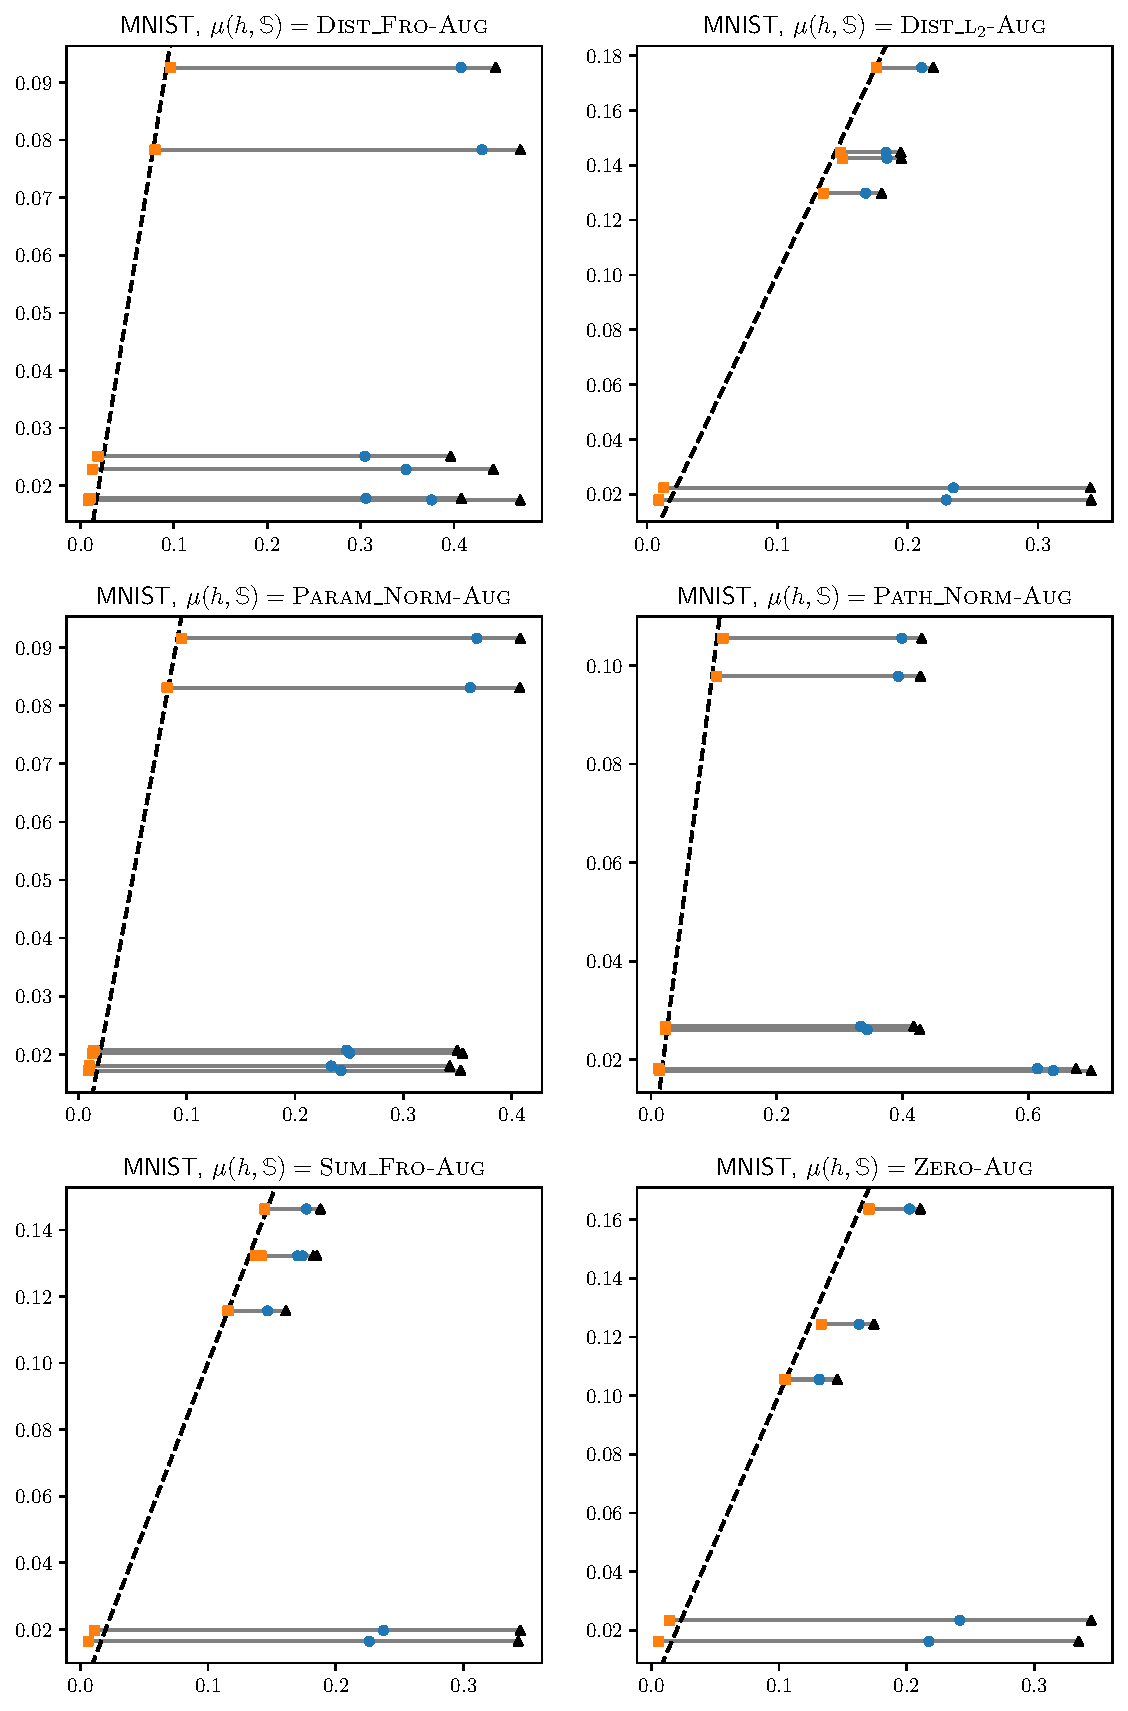
\includegraphics[width=0.77\linewidth]{chapter_7/figures/gap_mnist_aug.pdf}
    \caption{
    \looseness=-1
    Scatter plot given a parametric function $\comp(\h, \S)$, where each segment represents a neural network $\h_{\wbf}$ learned with a given $\alpha$, width $H$ and depth $L$.
    For each segment, there is a corresponding orange square and a blue circle.
    The orange squares corresponds to the empirical risk $\Risk_{\dS}(\h)$ (x-axis) and test risk $\Risk_{\dT}(\h)$ (y-axis).
    The blue circle \resp the black triangle represents \Cref{chap:dis-mu:eq:disintegrated-comp-seeger-risk} \resp \Cref{chap:dis-mu:eq:disintegrated-comp-mcallester-risk} in the x-axis and the test risk $\Risk_{\dT}(\h)$ in the y-axis.
    The dashed line is the identity function.
    }
    \label{chap:dis-mu:fig:gap-mnist-aug}
\end{figure}

\begin{figure}
    \centering
    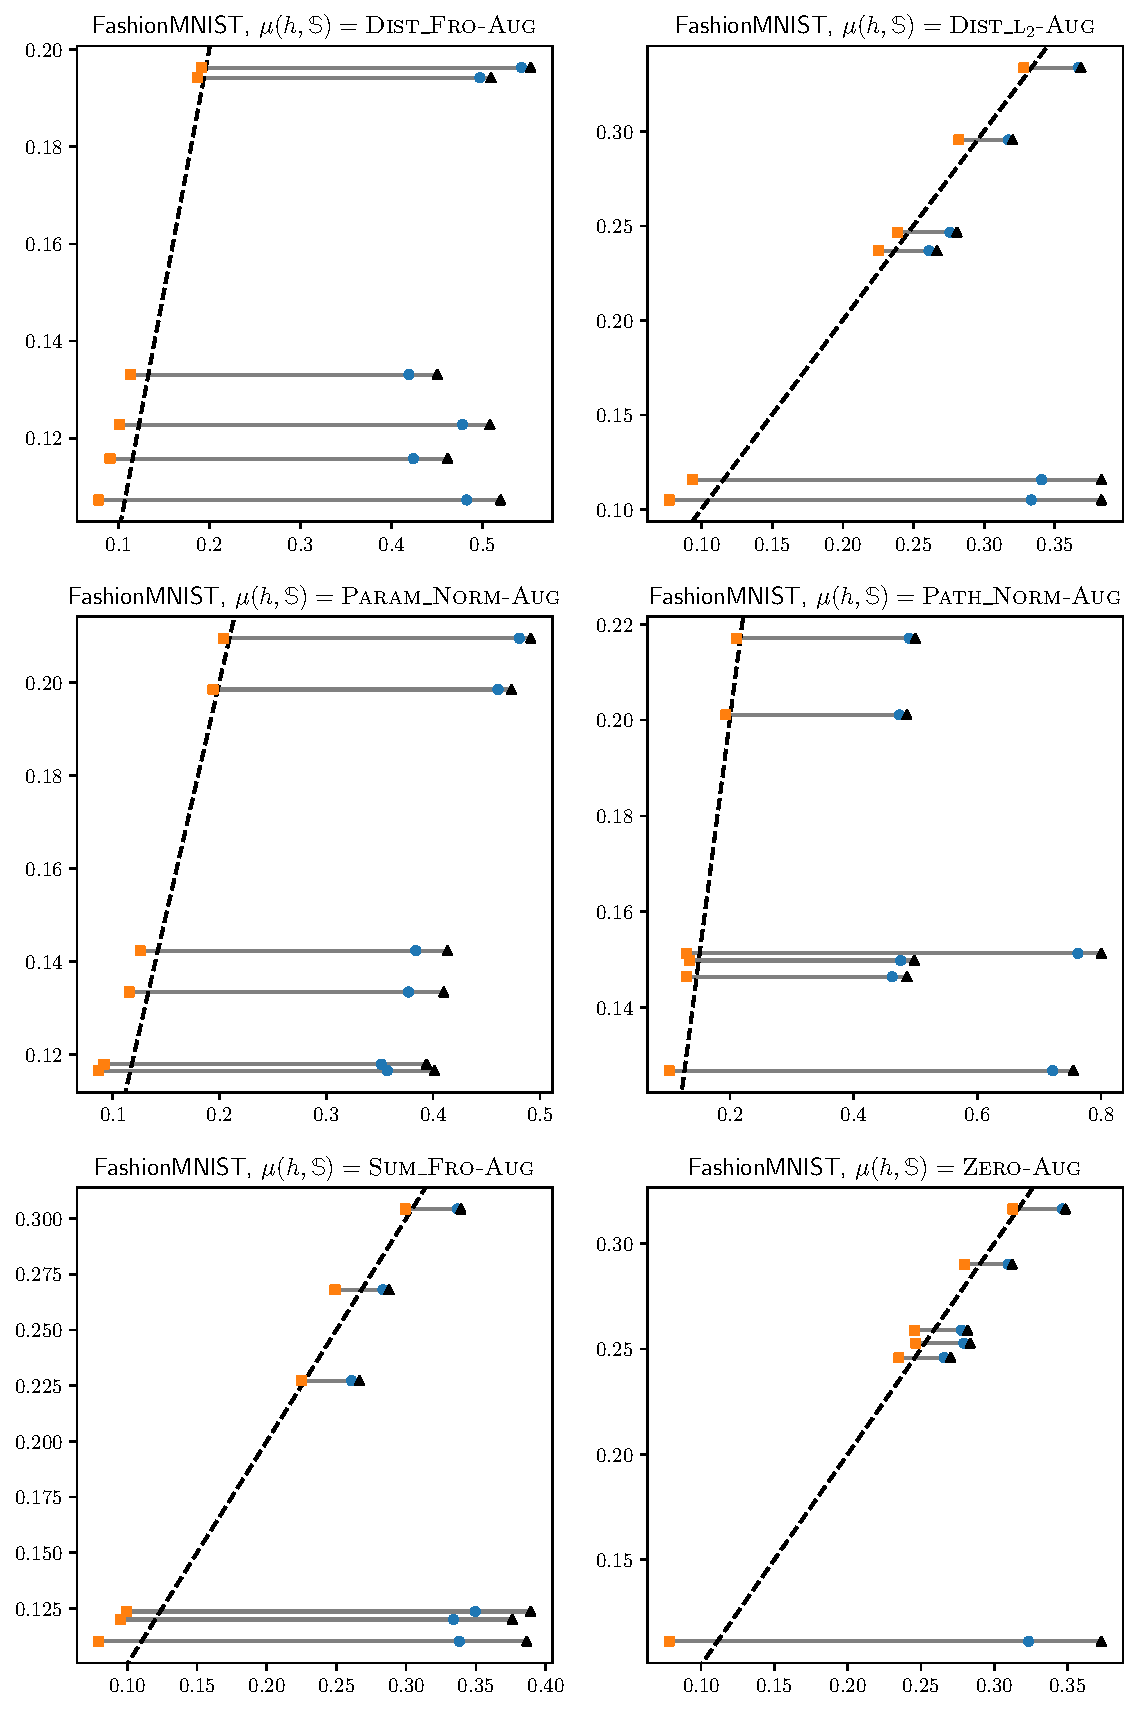
\includegraphics[width=0.77\linewidth]{chapter_7/figures/gap_fashion_aug.pdf}
    \caption{
    \looseness=-1
    Scatter plot given a parametric function $\comp(\h, \S)$, where each segment represents a neural network $\h_{\wbf}$ learned with a given $\alpha$, width $H$ and depth $L$.
    For each segment, there is a corresponding orange square and a blue circle.
    The orange squares corresponds to the empirical risk $\Risk_{\dS}(\h)$ (x-axis) and test risk $\Risk_{\dT}(\h)$ (y-axis).
    The blue circle \resp the black triangle represents \Cref{chap:dis-mu:eq:disintegrated-comp-seeger-risk} \resp \Cref{chap:dis-mu:eq:disintegrated-comp-mcallester-risk} in the x-axis and the test risk $\Risk_{\dT}(\h)$ in the y-axis.
    The dashed line is the identity function.
    }
    \label{chap:dis-mu:fig:gap-fashion-aug}
\end{figure}

\subsection{Influence of the Parameter $\alpha$}

\Cref{ap:dis-mu:fig:influence-alpha-1,ap:dis-mu:fig:influence-alpha-2,ap:dis-mu:fig:influence-alpha-3,ap:dis-mu:fig:influence-alpha-4} shows the influence of the parameter $\alpha$ for all parametric functions.

\begin{figure}
    \centering
    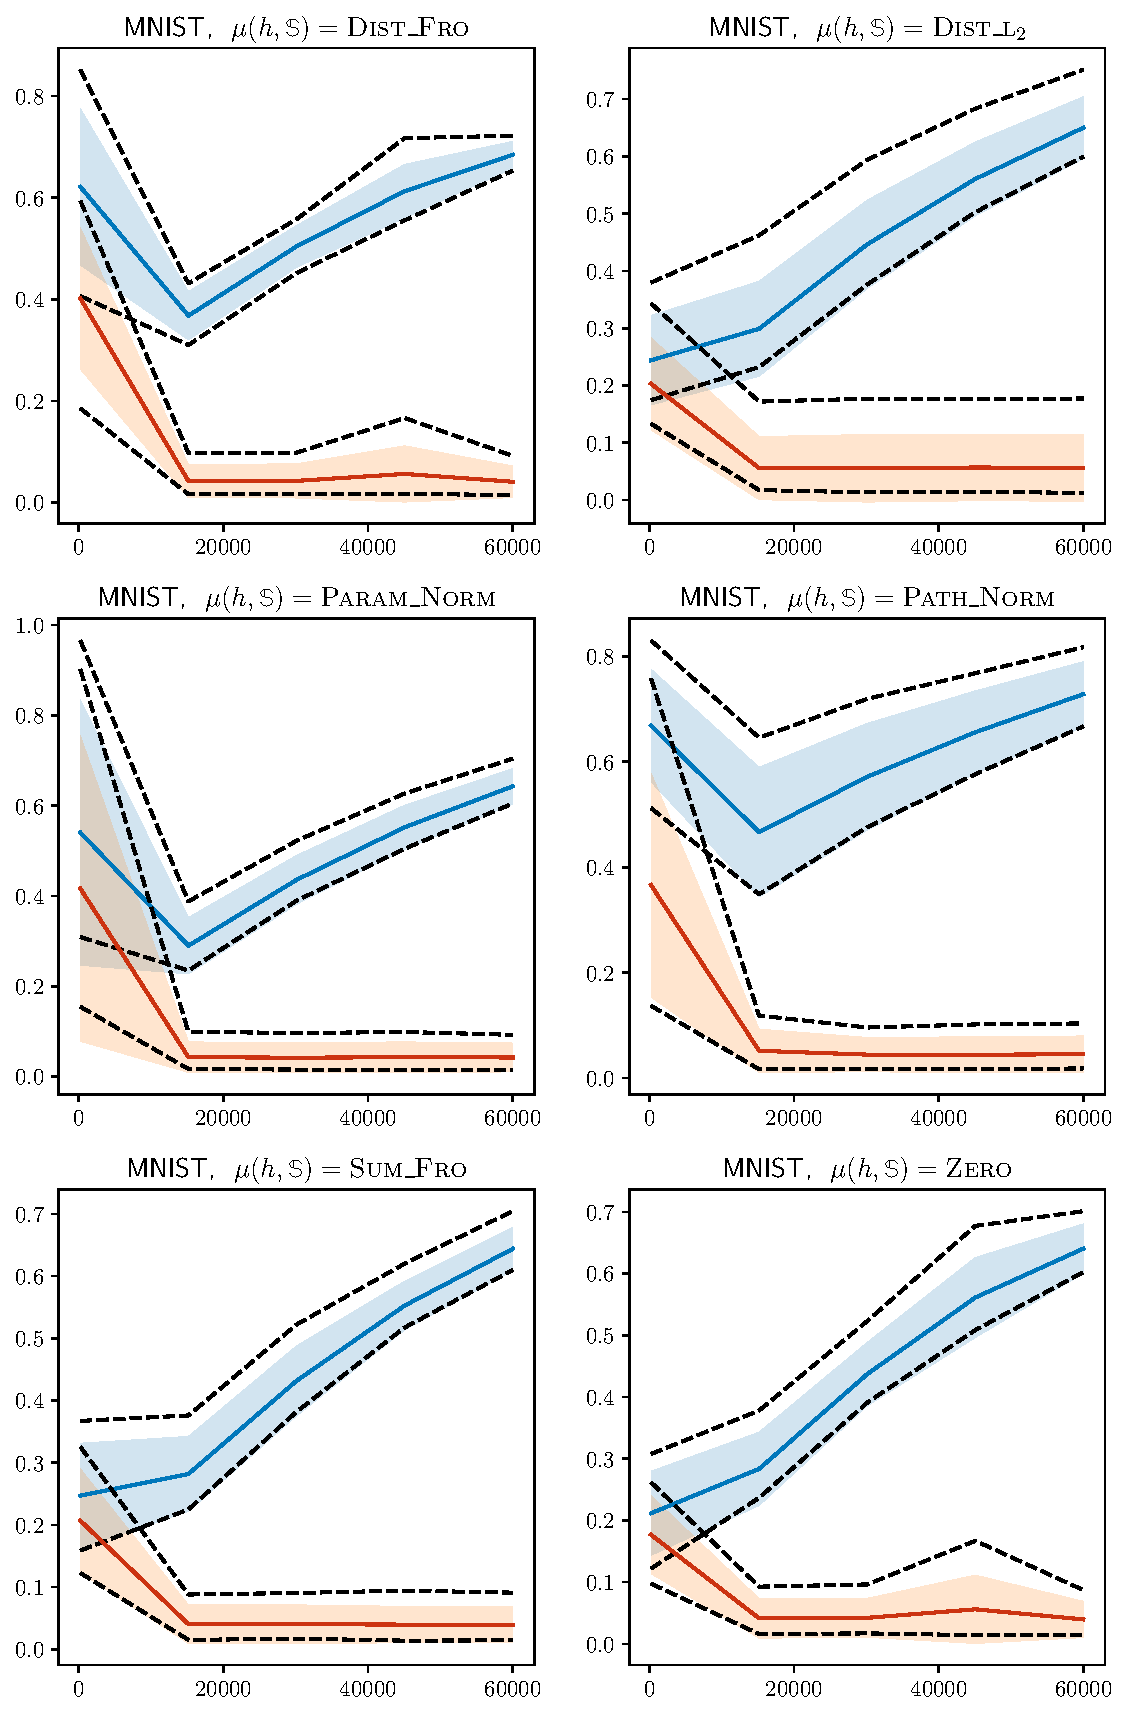
\includegraphics[width=0.77\linewidth]{chapter_7/figures/influence_alpha_mnist.pdf}
    \caption{
    Influence of the parameter $\alpha$ in the x-axis.
    The bound values are represented in blue and the test risk in red. 
    The two (solid) lines are the mean values computed on the depths and widths; the shadows are the standard deviation.
    The dashed lines are the minimum and the maximum values.
    }
    \label{ap:dis-mu:fig:influence-alpha-1}
\end{figure}

\begin{figure}
    \centering
    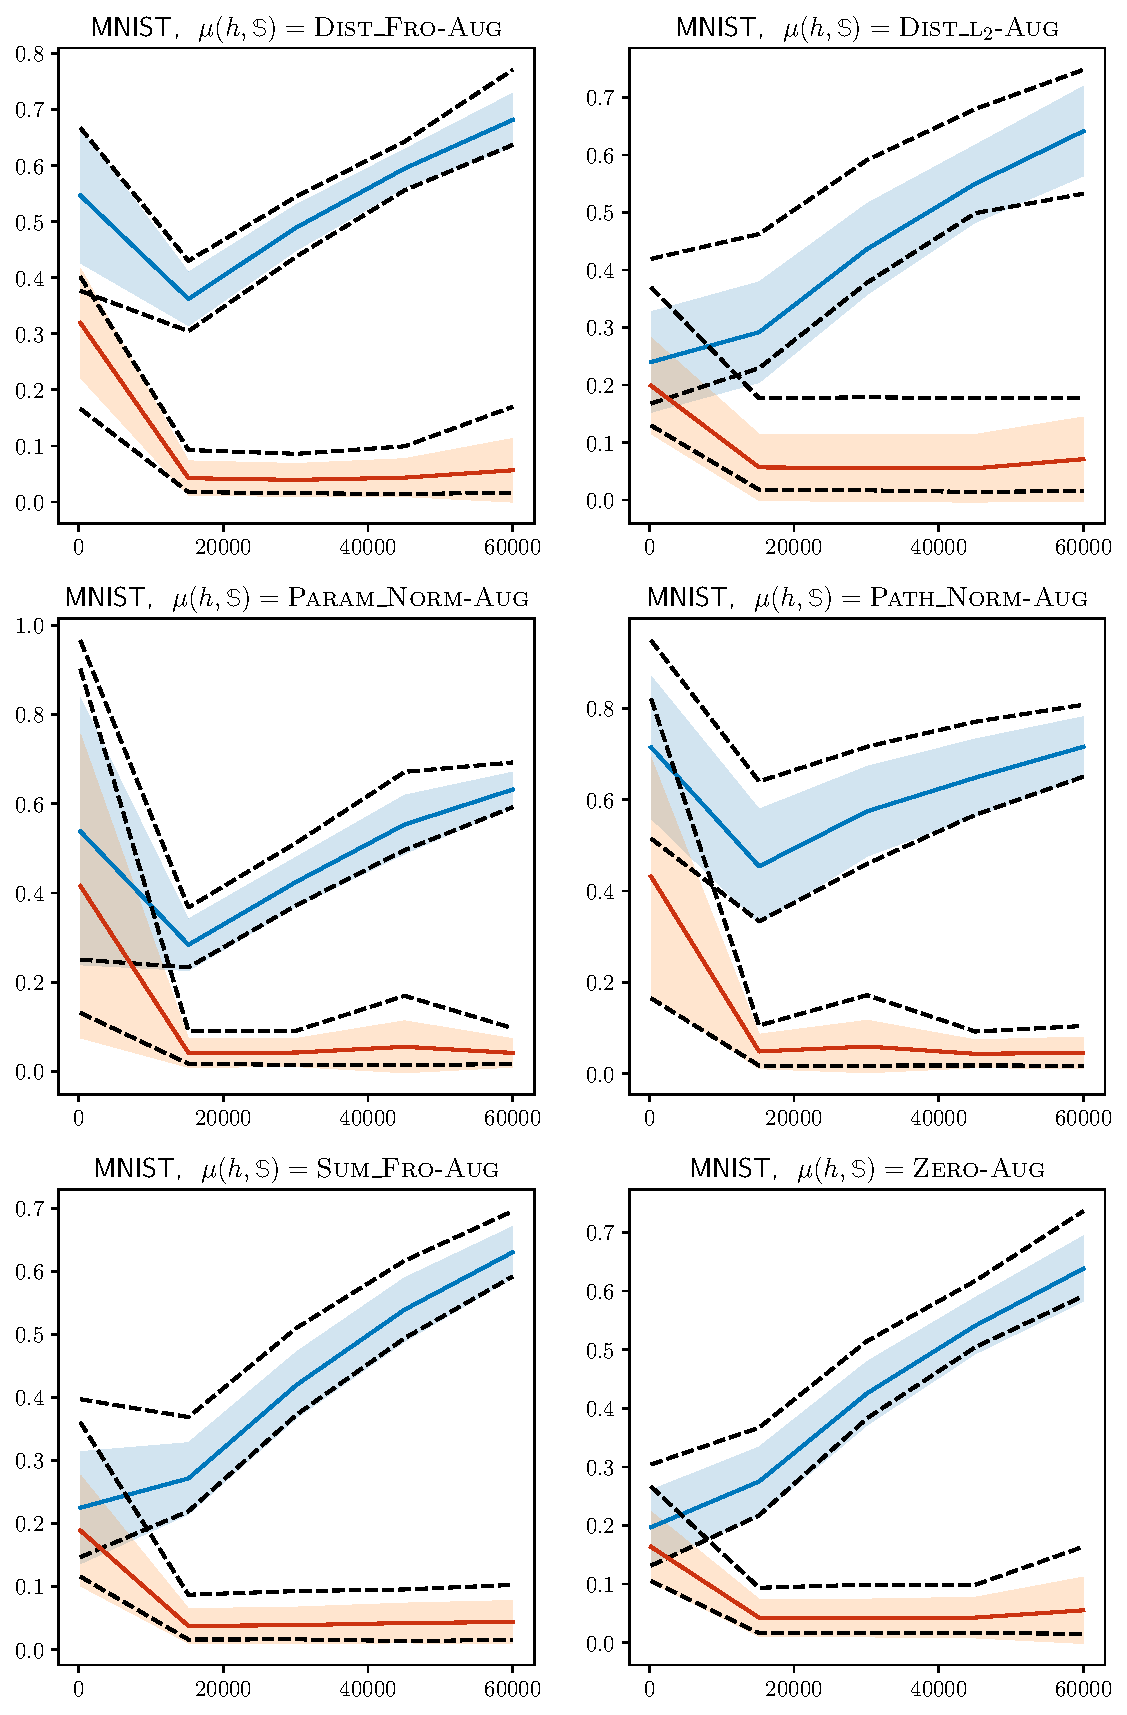
\includegraphics[width=0.77\linewidth]{chapter_7/figures/influence_alpha_mnist_aug.pdf}
    \caption{
    Influence of the parameter $\alpha$ in the x-axis.
    The bound values are represented in blue and the test risk in red. 
    The two (solid) lines are the mean values computed on the depths and widths; the shadows are the standard deviation.
    The dashed lines are the minimum and the maximum values.
    }
    \label{ap:dis-mu:fig:influence-alpha-2}
\end{figure}

\begin{figure}
    \centering
    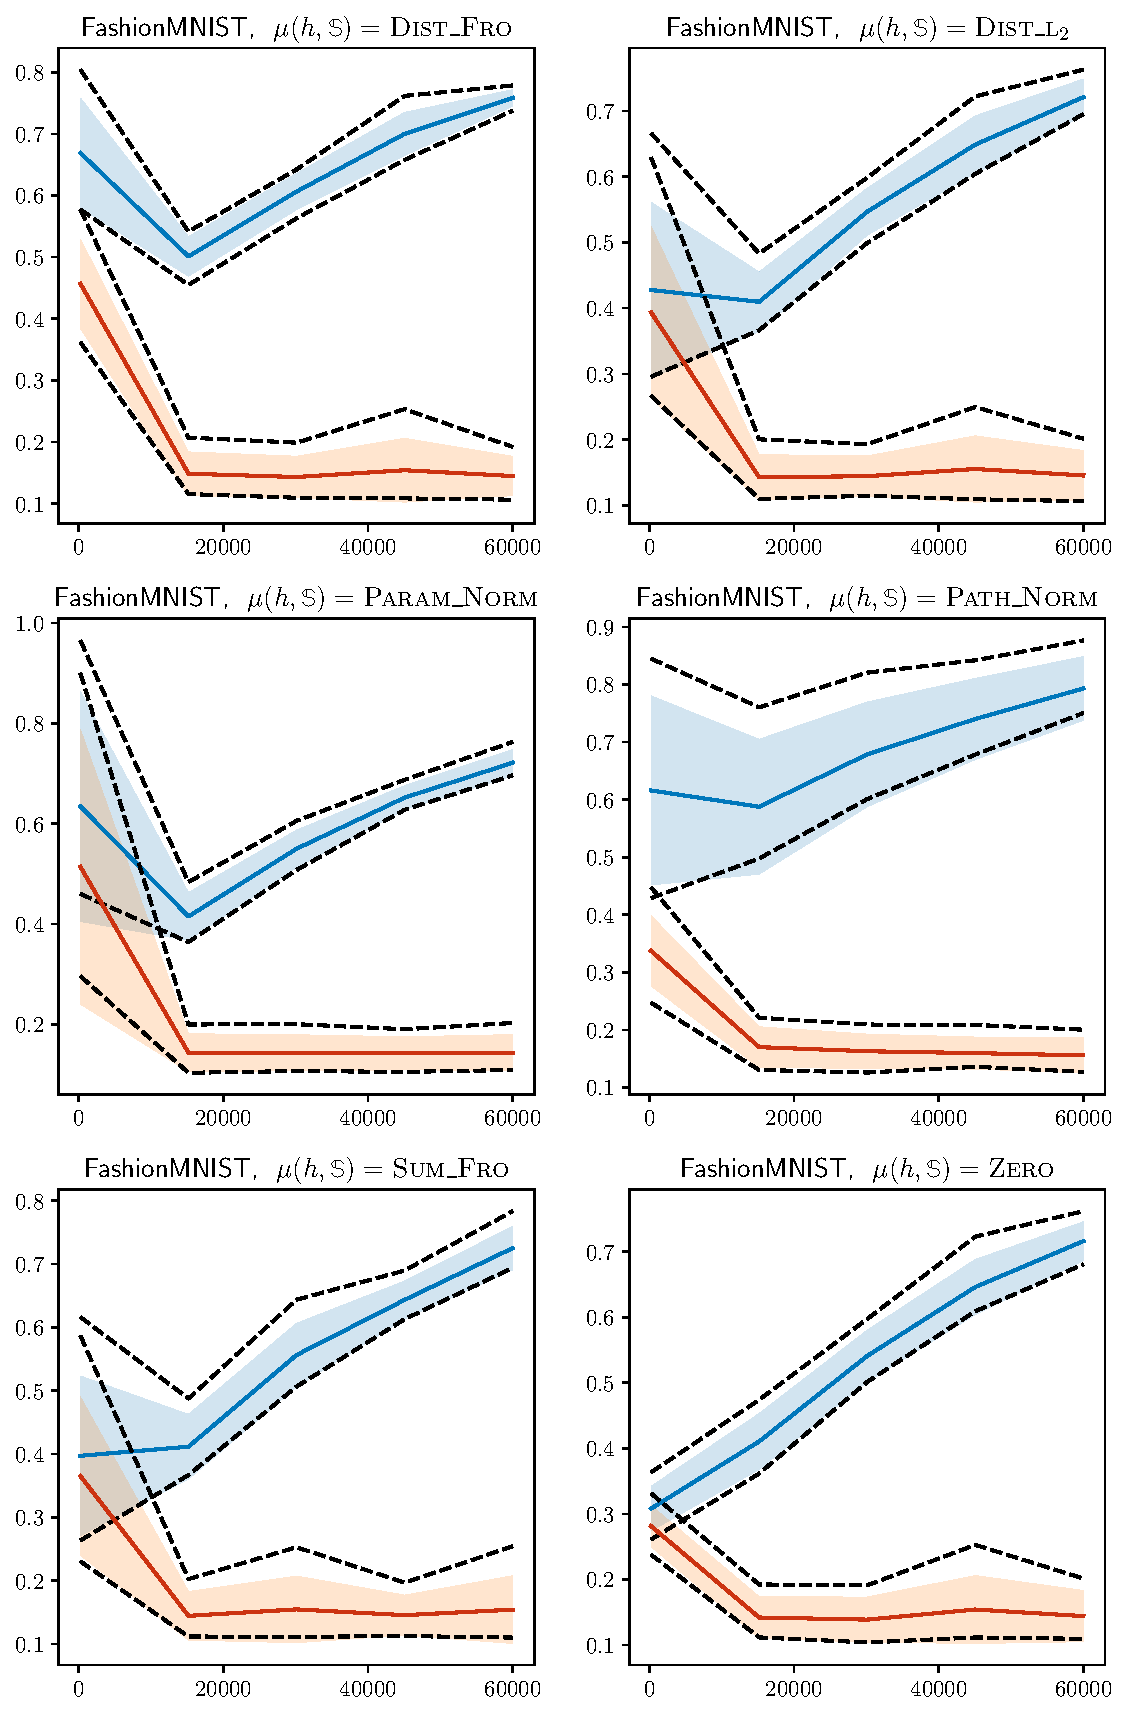
\includegraphics[width=0.77\linewidth]{chapter_7/figures/influence_alpha_fashion.pdf}
    \caption{
    Influence of the parameter $\alpha$ in the x-axis.
    The bound values are represented in blue and the test risk in red. 
    The two (solid) lines are the mean values computed on the depths and widths; the shadows are the standard deviation.
    The dashed lines are the minimum and the maximum values.
    }
    \label{ap:dis-mu:fig:influence-alpha-3}
\end{figure}

\begin{figure}
    \centering
    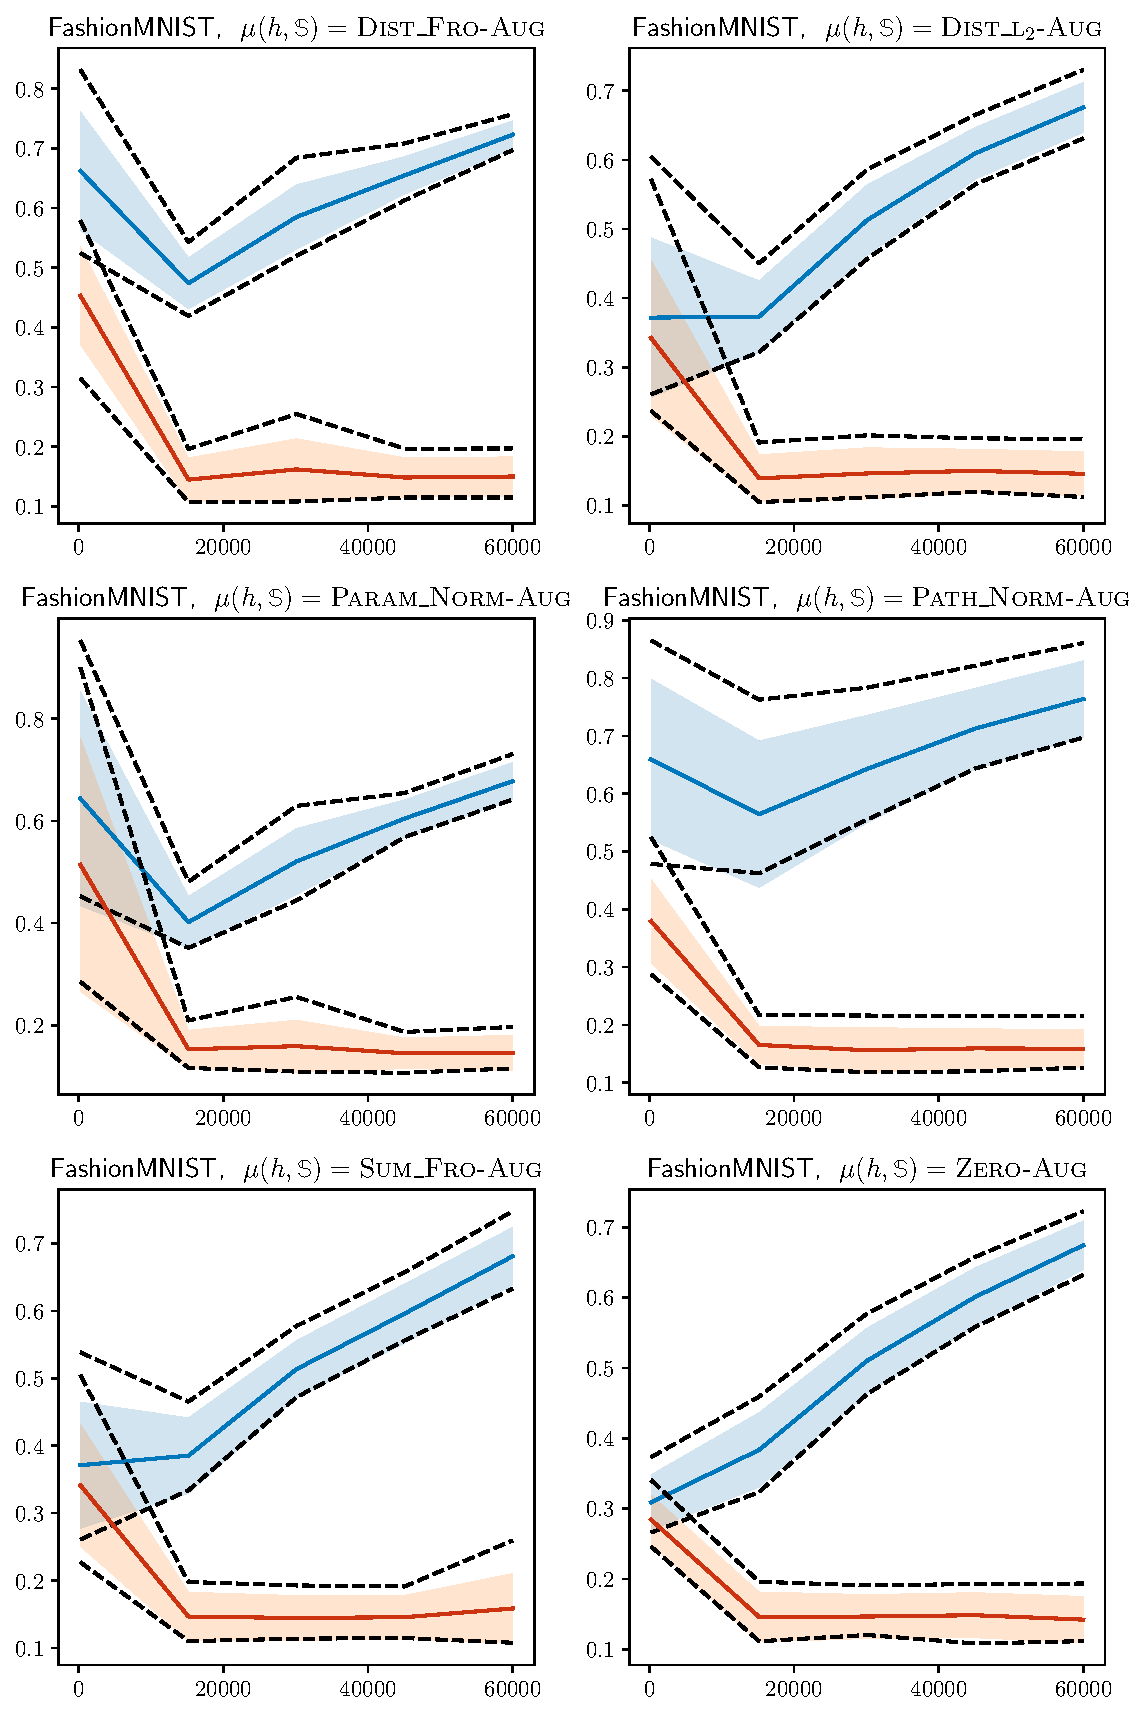
\includegraphics[width=0.77\linewidth]{chapter_7/figures/influence_alpha_fashion_aug.pdf}
    \caption{
    Influence of the parameter $\alpha$ in the x-axis.
    The bound values are represented in blue and the test risk in red. 
    The two (solid) lines are the mean values computed on the depths and widths; the shadows are the standard deviation.
    The dashed lines are the minimum and the maximum values.
    }
    \label{ap:dis-mu:fig:influence-alpha-4}
\end{figure}

\subsection{Influence of the Depth/Width}

\Cref{ap:dis-mu:fig:influence-depth-1,ap:dis-mu:fig:influence-depth-2,ap:dis-mu:fig:influence-depth-3,ap:dis-mu:fig:influence-depth-4} shows the influence of the depth and the width for all parametric functions.

\begin{figure}
    \centering
    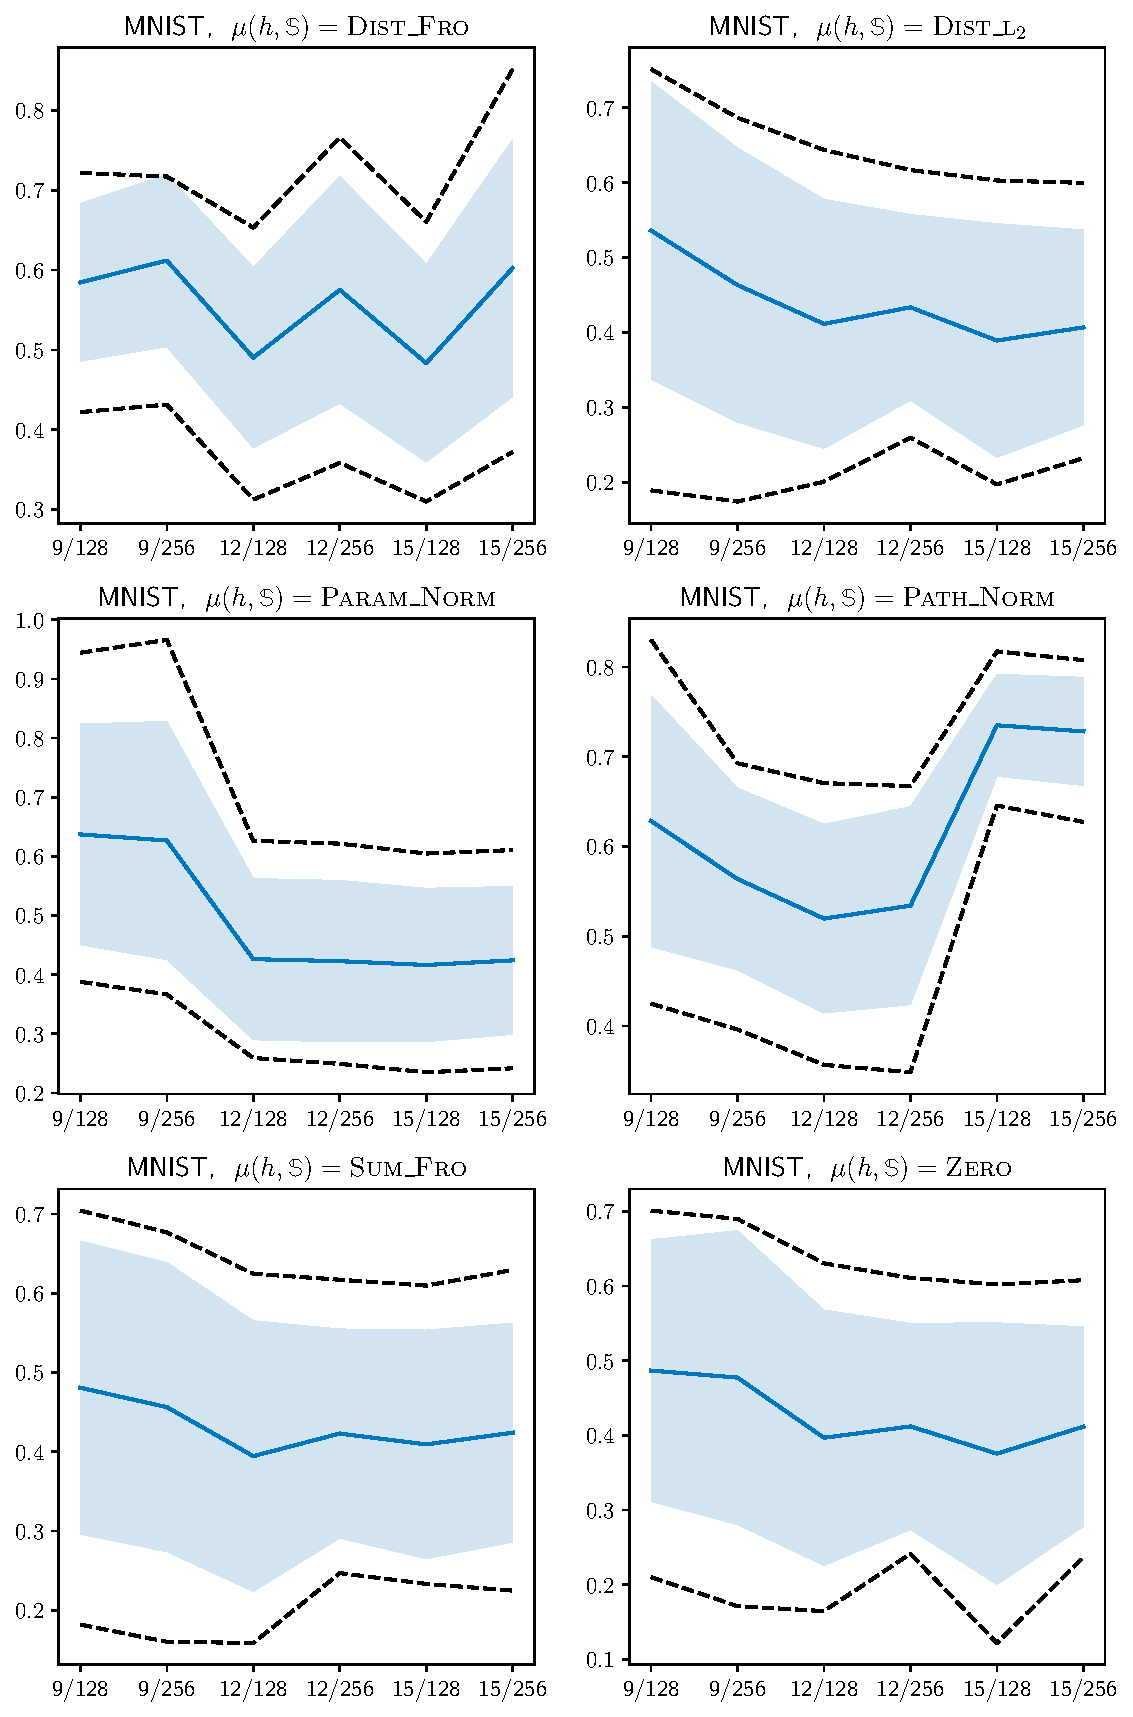
\includegraphics[width=0.77\linewidth]{chapter_7/figures/influence_depth_mnist.pdf}
    \caption{
    Influence of the depth and the width in the x-axis as ``depth/width''.
    The (solid) lines are the mean values computed on the different values of $\alpha$; the shadows are the standard deviation. 
    The dashed lines are the minimum and the maximum values.
    }
    \label{ap:dis-mu:fig:influence-depth-1}
\end{figure}

\begin{figure}
    \centering
    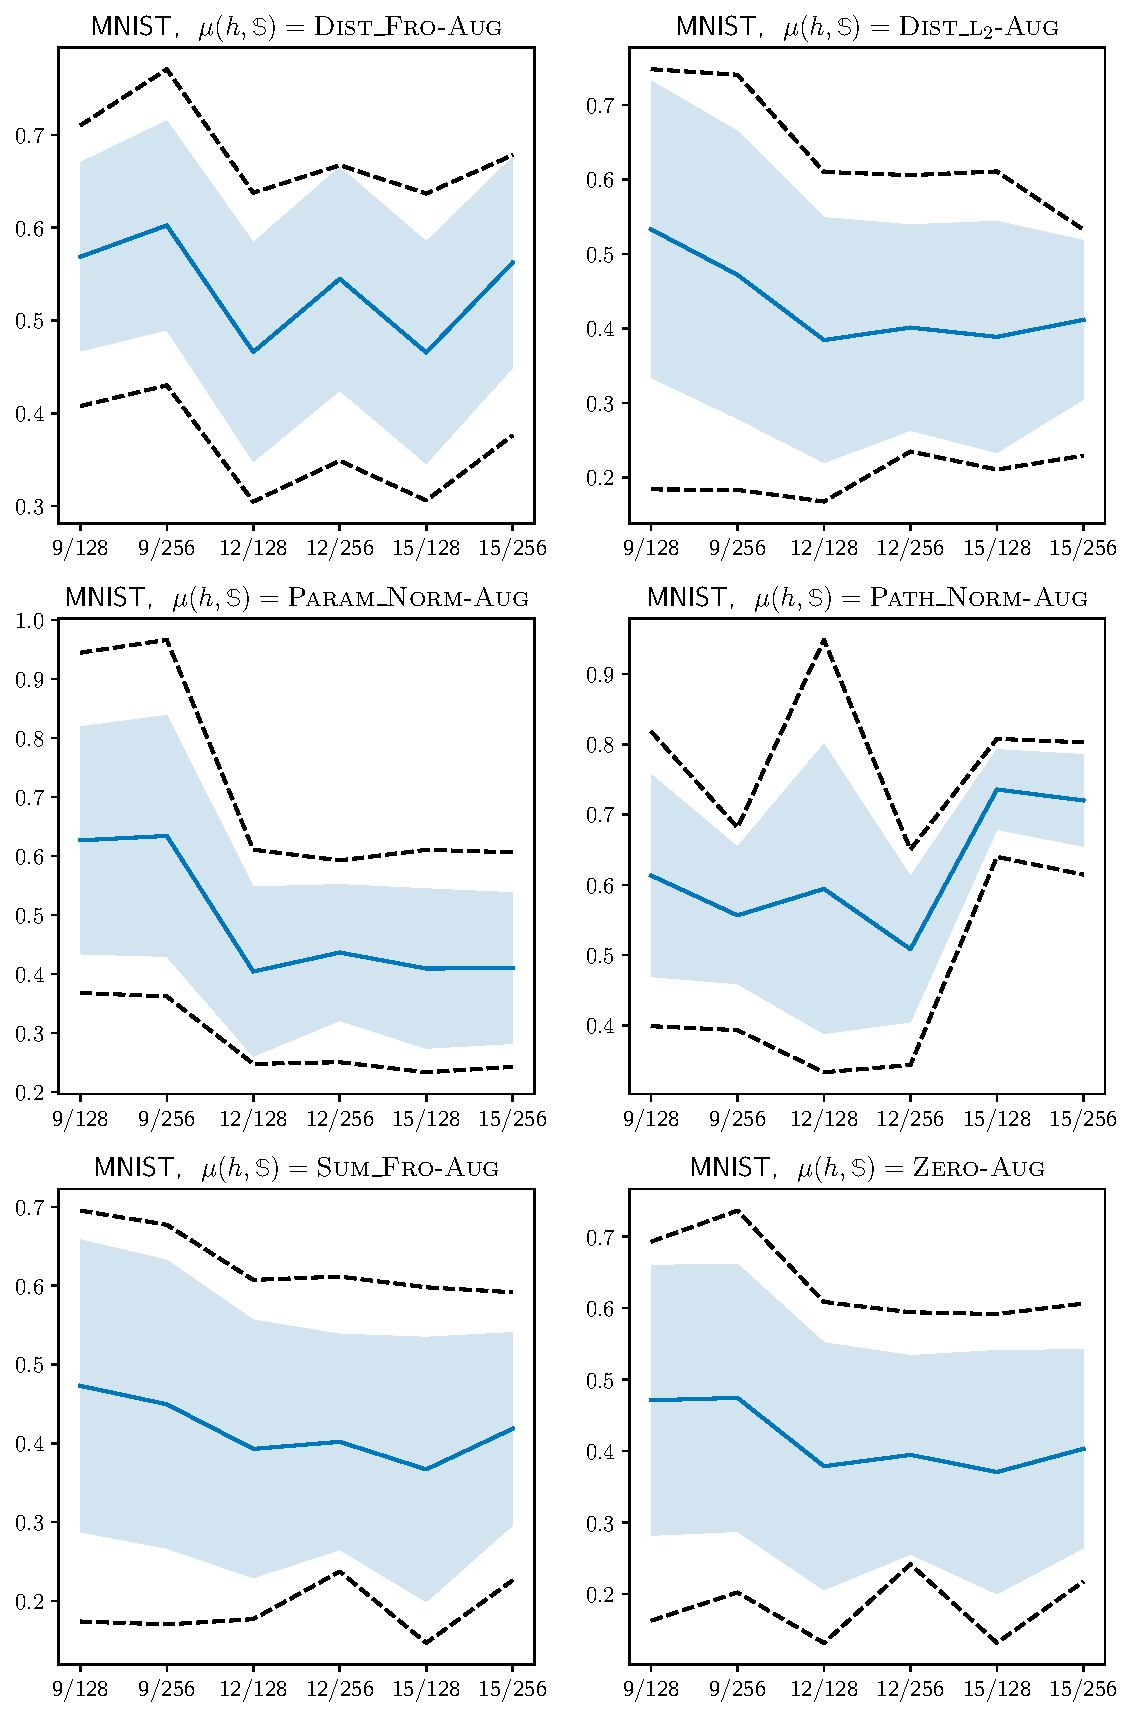
\includegraphics[width=0.77\linewidth]{chapter_7/figures/influence_depth_mnist_aug.pdf}
    \caption{
    Influence of the depth and the width in the x-axis as ``depth/width''.
    The (solid) lines are the mean values computed on the different values of $\alpha$; the shadows are the standard deviation. 
    The dashed lines are the minimum and the maximum values.
    }
    \label{ap:dis-mu:fig:influence-depth-2}
\end{figure}

\begin{figure}
    \centering
    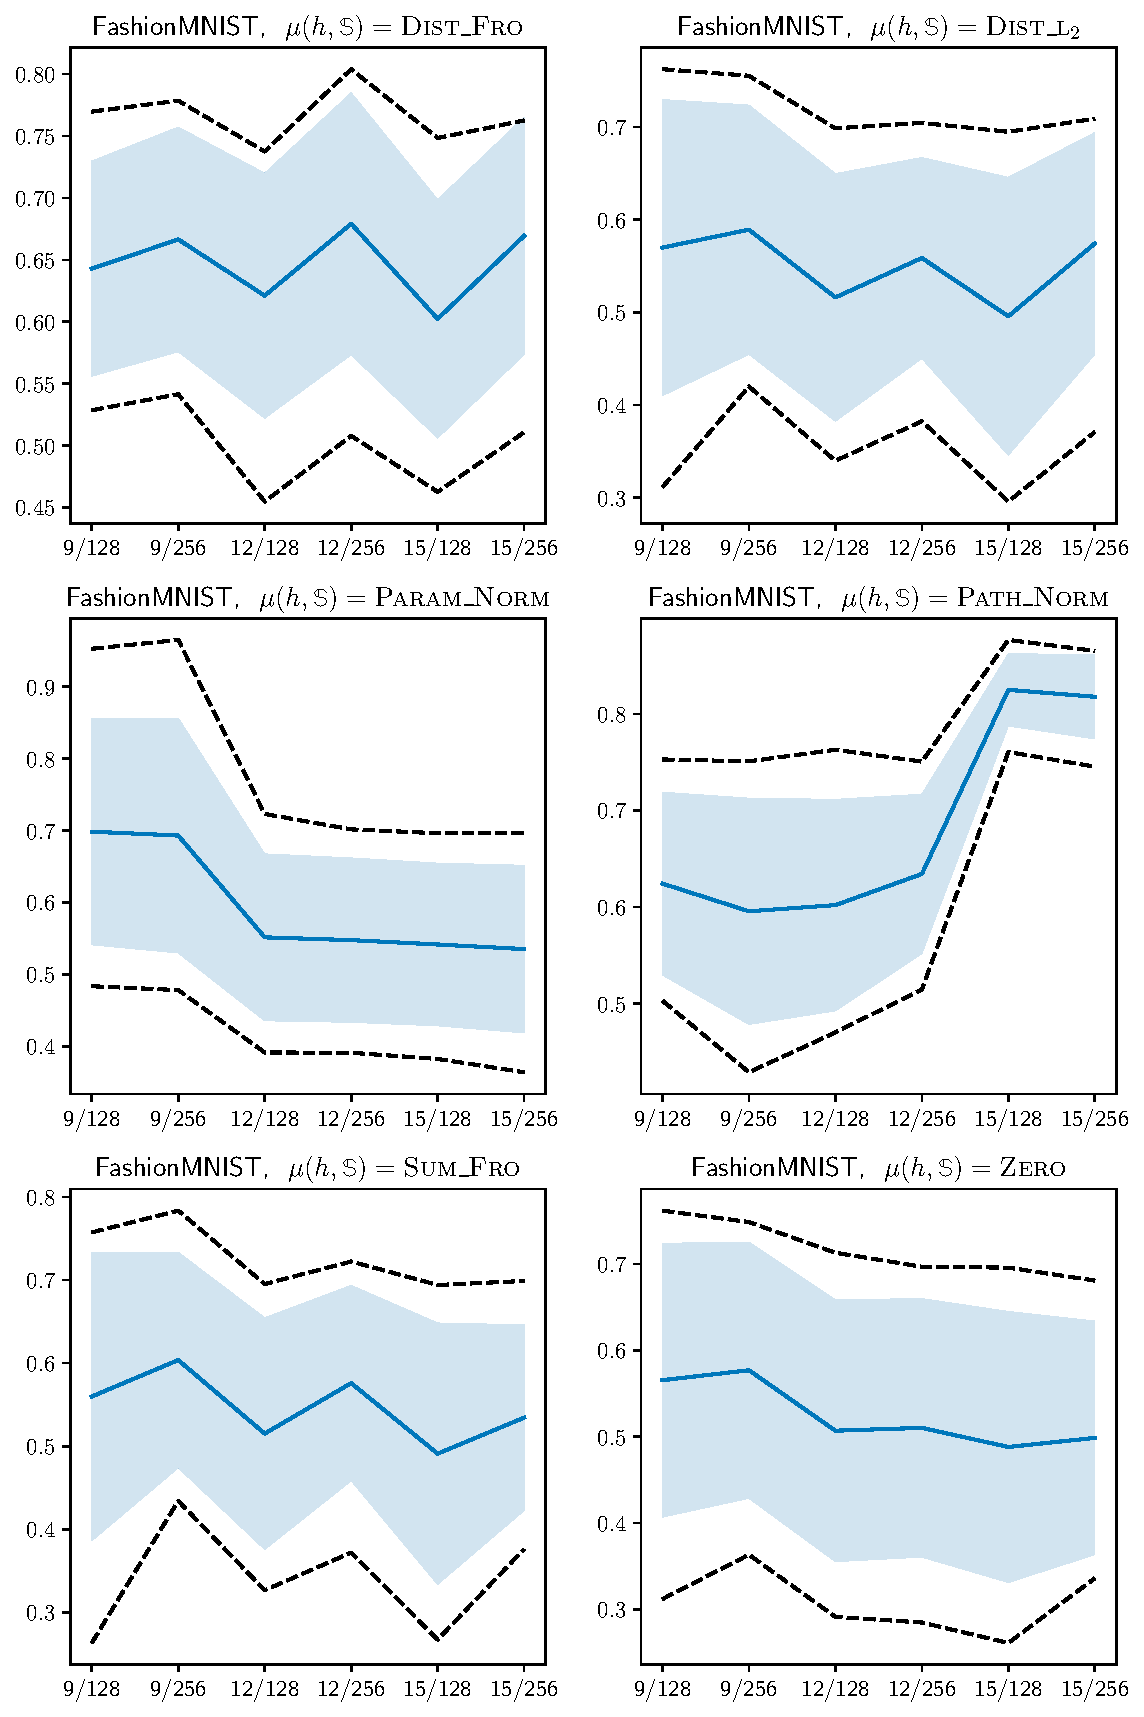
\includegraphics[width=0.77\linewidth]{chapter_7/figures/influence_depth_fashion.pdf}
    \caption{
    Influence of the depth and the width in the x-axis as ``depth/width''.
    The (solid) lines are the mean values computed on the different values of $\alpha$; the shadows are the standard deviation. 
    The dashed lines are the minimum and the maximum values.
    }
    \label{ap:dis-mu:fig:influence-depth-3}
\end{figure}

\begin{figure}
    \centering
    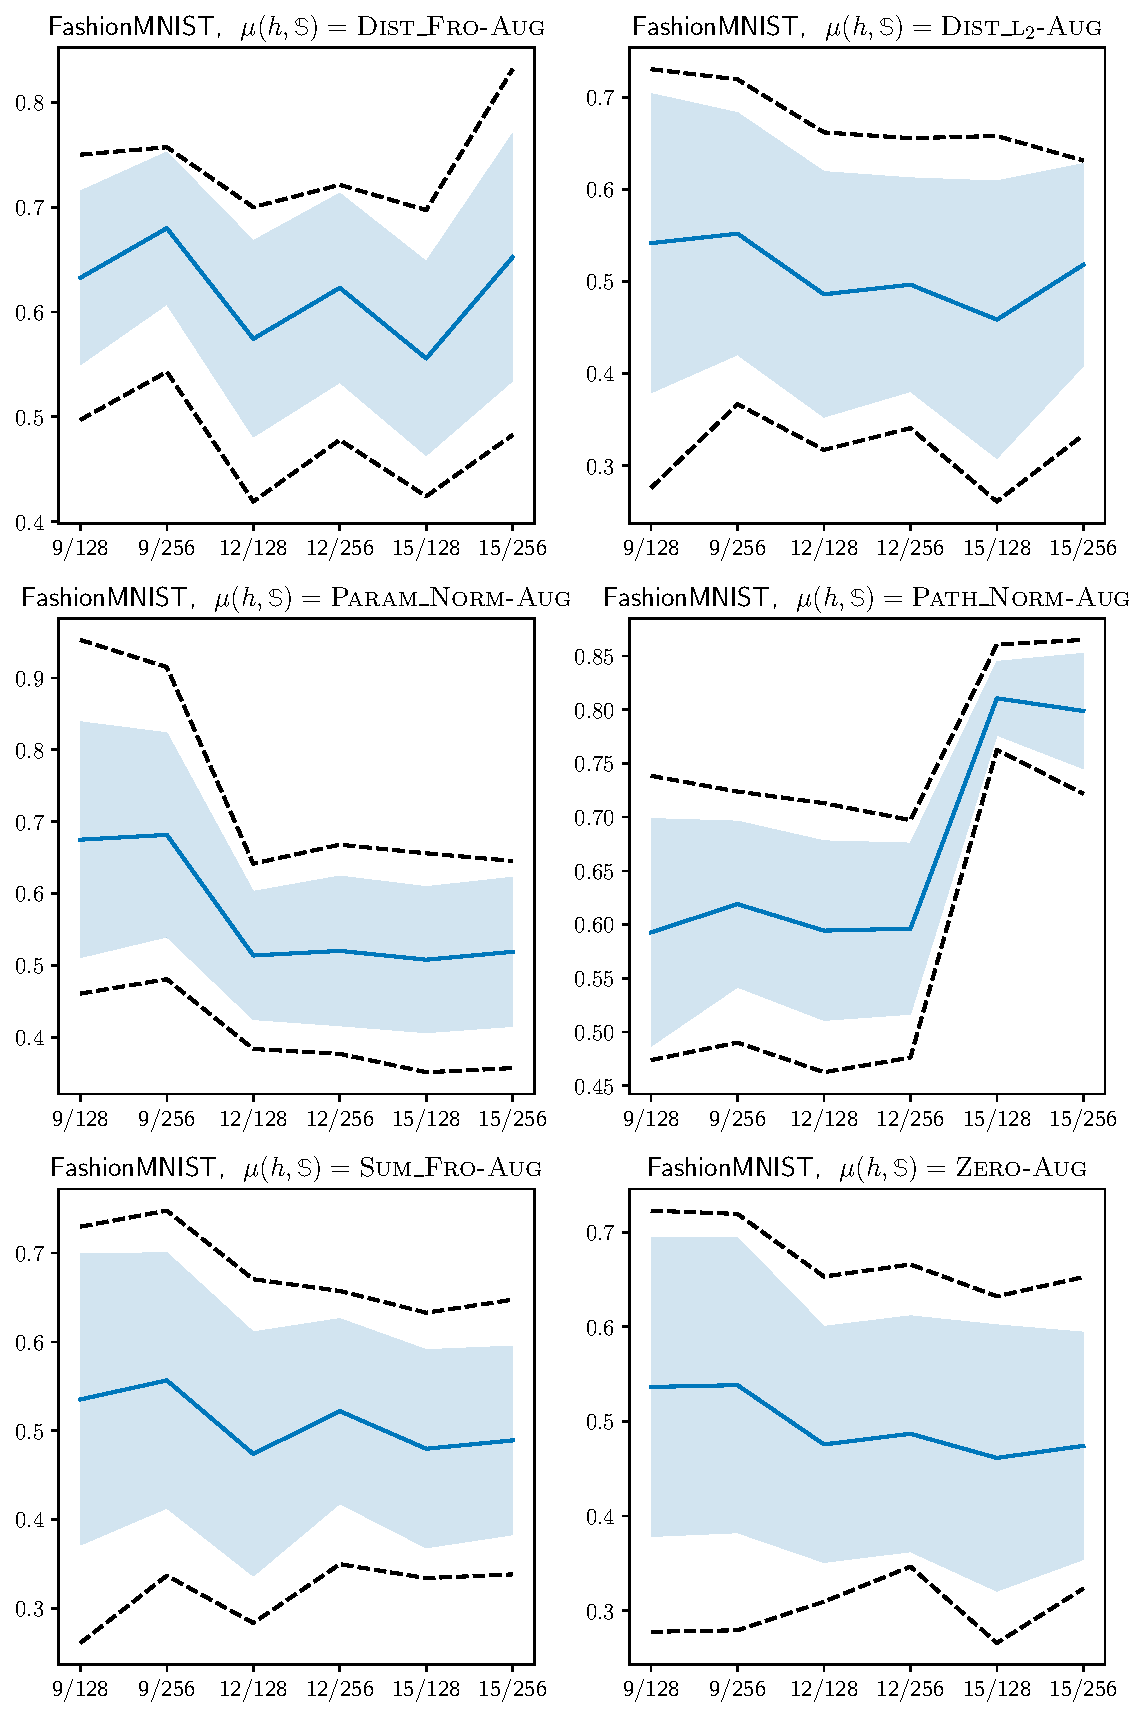
\includegraphics[width=0.77\linewidth]{chapter_7/figures/influence_depth_fashion_aug.pdf}
    \caption{
    Influence of the depth and the width in the x-axis as ``depth/width''.
    The (solid) lines are the mean values computed on the different values of $\alpha$; the shadows are the standard deviation. 
    The dashed lines are the minimum and the maximum values.
    }
    \label{ap:dis-mu:fig:influence-depth-4}
\end{figure}
\end{noaddcontents}